\section{Experimental evaluation}\label{sec:experimental-evaluation}

\subsection{Experiment setup}

\subsubsection{Datasets}

The proposed methods were experimentally verified on several datasets. The datasets Cora and CiteSeer \cite{yang_revisiting_2016} were used with the \enquote{full} train-test split as in \cite{chen_fastgcn_2018}. In addition, 2 variants of the Twitch dataset \cite{rozemberczki_multi-scale_2021} with the hignest node count (DE and EN) were used. Five medium sized datasets were also used, the PubMed dataset \cite{yang_revisiting_2016}, the DBLP dataset \cite{bojchevski_deep_2018}, the IMDB dataset \cite{xinyu_magnn:_2020} and both variants of the Coauthor dataset \cite{shchur_pitfalls_2019}. Finally, one large dataset was used, the OGB ArXiv dataset \cite{weihua_open_2021}.

\subsubsection{Methodology of experiments}

The hyper-parameters for both the node2vec model used for the embedding training and the multi-layer perceptron used for downstream classification were initially set to values used in prior art (see \cite{hu_open_2021,fey_fast_2019}) and then manually fine-tuned for each dataset.

The achitecture of the algorithm was identical accross the dataset, with the only difference being in the values of the hyper-parameters, as listed in Table~\ref{tab:hyperparameter-values}. For the Cora dataset, the node2vec model generated an embedding in \( \mathfield{R}^{128} \) from \( 4 \) random walks of length \( 20 \) for each node with a context window of size \( 5 \). The optimizer ADAM \cite{kingma_adam:_2017} was used with a learning rate of \( 0.01 \) and batches of \( 128 \) samples. The model was trained for \( 5 \) epochs and in each step of the adaptive prolongation, \( 100 \) nodes were prolonged, until reaching the original graph (the value of \( n_p \) was calculated so that the total number of training epochs would match baseline model training). The MLP classifier using the embeddings featured \( 3 \) linear layers of \( 128 \) neurons with batch normalization after each layer. Each layer was normalized using dropout \cite{srivastava_dropout_2014} with the rate of \( 0.5 \). Finally, a linear layer was used for the class prediction. For the classifier, ADAM with a learning rate of \( 0.01 \) was used for \( 30 \) epochs of training with the cross-entropy loss function. Dataset features weren't used for the classifier training as the aim of this work is to compare the embeddings. The experiment was run \( 10 \) times end-to-end and results averaged. The experiments were implemented using PyTorch \cite{paszke_pytorch_2019} and PyTorch Geometric \cite{fey_fast_2019}.

\begin{table*}
  \caption{Hyper-parameter values used for different datasets}
  \label{tab:hyperparameter-values}
  \centering
  \begin{adjustbox}{max width=\textwidth}
    \begin{tabular}{lrrrrrrrr}
      \toprule
      \textbf{Hyper-parameter} & \textbf{Cora} & \textbf{CiteSeer} & \textbf{PubMed} & \textbf{DBLP} & \textbf{Twitch} & \textbf{IMDB} & \textbf{ArXiv} & \textbf{Coauthor} \\
      \midrule
      Embedding dimension      & 128           & 32                & 64              & 32            & 128             & 128           & 128            & 128               \\
      \# of random walks       & 4             & 5                 & 3               & 2             & 10              & 40            & 10             & 40                \\
      Random walk length       & 20            & 20                & 40              & 20            & 80              & 100           & 80             & 10                \\
      Context window size      & 5             & 5                 & 20              & 5             & 3               & 5             & 20             & 5                 \\
      Node2vec learning rate   & 0.01          & 0.01              & 0.01            & 0.01          & 0.025           & 0.01          & 0.01           & 0.01              \\
      Node2vec batch size      & 128           & 128               & 128             & 128           & 128             & 256           & 128            & 256               \\
      Node2vec epochs          & 5             & 7                 & 1               & 1             & 5               & 1             & 1              & 1                 \\
      %\# of prolonged nodes    & 100           & 150               & 1000            & 800           & 200             & 1400          & 8000           & 1250              \\
      \# of MLP layers         & 3             & 3                 & 1               & 3             & 2               & 2             & 3              & 2                 \\
      MLP hidden layer width   & 128           & 256               & 128             & 256           & 64              & 64            & 256            & 16                \\
      Dropout rate             & 0.5           & 0.5               & 0.5             & 0.5           & 0.5             & 0.5           & 0.5            & 0.5               \\
      MLP learning rate        & 0.01          & 0.01              & 0.01            & 0.01          & 0.01            & 0.01          & 0.01           & 0.01              \\
      MLP epochs               & 30            & 80                & 300             & 300           & 500             & 100           & 300            & 100               \\
      \bottomrule
    \end{tabular}
  \end{adjustbox}
\end{table*}

\subsection{Evaluation of the adaptive approach}\label{sec:adaptive-experiments}

In order to study the effect of the adaptive prolongation, the adaptive prolongation method was used to assess the performance of downstream transductive classification at different coarsening levels. A node2vec model as described in the previous section was trained with adaptive prolongation based on coarsenings pre-computed by the HARP coarsening algorithm as described in \ref{sec:harp-coarsening}. For each prolongation step, the intermediary embedding was afterwards fully prolonged to obtain an embedding of the original graph \( G \) (as that is the only graph for which ground-truth labels are available). A classifier was then trained with this embedding as input. This setup allows us to compare classification accuracy at each step of the adaptive prolongation. Figure~\ref{fig:adaptive-coarsening} shows the results of this experiment, compared with a baseline node2vec model (that is, without any coarsening or prolongation) that was trained for the same number of epochs as the total epochs of the adaptive model over all prolongation steps.

\begin{figure*}
  \centering
  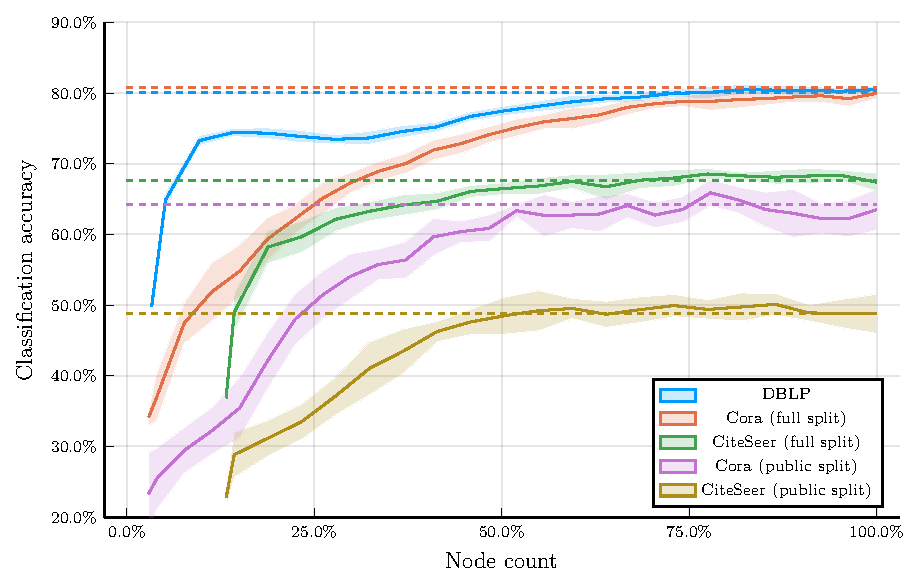
\includegraphics[width = \linewidth]{images/adaptive-coarsening/adaptive-coarsening.pdf}
  \caption{Downstream classifier accuracies at different steps of adaptive prolongation using the basic HARP coarsening algorithm. Dashed line shows the baseline node2vec model accuracy. The node count is taken relative to the total node count in each dataset. The results are averaged over multiple runs, with the solid line representing the mean and the shaded area denoting one standard deviation.}
  \label{fig:adaptive-coarsening}
\end{figure*}

The behaviour of the model somewhat differs between the used datasets. For the Cora, CiteSeer, DBLP, PubMed, ArXiv and Coauthor datasets, the model starts from a very low performance, which quickly rises as the model trains for several prolongation steps. The model trained on CiteSeer attains performance comparable to the reference model when approximately half of all nodes are available to it. On the other hand, with e. g. Coauthor-CS, the model slowly approaches the reference model for the whole duration of training, only reaching comparable performance at a point where nearly the whole graph is available to it. Models trained on the two medium-sized datasets, DBLP and PubMed, exhibit a different behaviour in that they briefly reach a local maximum followed by a slight decrease in performance until finally approaching the performance of the reference model in a manner similar to the models trained on Cora and CiteSeer. The ArXiv dataset exhibits a similar behaviour to a lesser extent. This behaviour is further discussed in the next section. The Twitch and IMDB datasets are substantially different, with very high initial performance and only small performance gains with increasing number of nodes available, with different variants of it exhibiting this effect to a different magnitude.

To further study the model properties from a statistical point of view, the results were evaluated at \( k \)-th deciles of the node count of the full graph, for all possible values of \( k \). At each decile, the performance of the model was compared to the baseline node2vec model using the Wilcoxon signed-rank test with the Holm-Bonferroni correction for multiple hypothesis testing with the hypothesis that the models are equivalent. The hypotheses were rejected by the test at the 5\% level of significance for \( k \in \left\{ 1, 2, 3, 4, 5 \right\} \), suggesting that the adaptive prolongation approach is valid and practically useful in situations where at least half of the nodes is available.

Following recent best-practice recommendations regarding verifying the statistical validity of results \cite{benavoli_time_2017}, the results were also studied from the point of view of Bayesian estimation. Similarly to the frequentist approach, the performance of the model was compared to that of the baseline model at \( k \)-th deciles of the node count, for all possible values of \( k \). The comparison was done using the Bayesian Wilcoxon signed-rank test \cite{benavoli_bayesian_2014} for 3 different widths of the region of practical equivalence (ROPE), 1\%, 5\% and 10\%. The probabilities that the two models are practically equivalent are listed in Table~\ref{tab:bayesian-adaptive}. Of a particular note is the fact that at 60\% complexity, the models have over a 99\% probability of being within 10 percentage points of performance -- showing that the proposed method may offer a significant complexity reduction in exchange for a relatively minor decrease in performance.

\begin{table}
  \caption{The probabilities that the adaptive approach will be practically equivalent to node2vec when compared on different fractions of the full graph and with different widths of the region of practical equivalence.}
  \label{tab:bayesian-adaptive}
  \centering
  \begin{tabular}{lrrr}
    \toprule
    \textbf{Nodes} & \textbf{1\% ROPE} & \textbf{5\% ROPE} & \textbf{10\% ROPE} \\
    \midrule
    \textbf{10\%}  & 0\%               & 0.3\%             & 2.5\%              \\
    \textbf{20\%}  & 0\%               & 0.8\%             & 14.1\%             \\
    \textbf{30\%}  & 0\%               & 1.7\%             & 35.3\%             \\
    \textbf{40\%}  & 0\%               & 5.3\%             & 72.0\%             \\
    \textbf{50\%}  & 0.1\%             & 35.3\%            & 85.7\%             \\
    \textbf{60\%}  & 0.6\%             & 62.2\%            & 99.7\%             \\
    \textbf{70\%}  & 32.0\%            & 84.7\%            & 100.0\%            \\
    \textbf{80\%}  & 30.0\%            & 99.9\%            & 100.0\%            \\
    \textbf{90\%}  & 48.9\%            & 100.0\%           & 100.0\%            \\
    \textbf{100\%} & 87.7\%            & 100.0\%           & 100.0\%            \\
    \bottomrule
  \end{tabular}
\end{table}

\subsection{The relationship of the results and the properties of the graph}

When the models for DBLP and PubMed are studied more closely, both reach a local maximum at around 14\% of the graph, followed by a slight decline and gradual approach to the baseline. This suggests a global structure in the data, which the model learns at the point of the local maxima. To investigate this hypothesis and try to explain the behaviour of the model in general, several graph metrics were applied to the graphs generated during the adaptive prolongation algorithm run. All of the metrics were applied to the graph \( G_i \) at each step in the prolongation process.

The metrics used were edge homophily \cite{zhu_beyond_2020}, node homophily \cite{pei_geom-gcn_2020}, class homophily \cite{lim_large_2021}, adjusted homophily \cite{platonov_characterizing_2022}, balanced accuracy \cite{platonov_characterizing_2022}, adjusted accuracy \cite{platonov_characterizing_2022}, label informativeness \cite{platonov_characterizing_2022}, and global assortativity \cite{newman_mixing_2003}.

The values of these metrics were compared to the classification accuracy and a strong correlation was found for the majority of them, with correlation coefficient of \( -0.66 \) for global assortativity and between \( 0.94 \) and \( 0.96 \) for all the other metrics, averaged across the datasets. This suggests the explanation of the graphs being heterophilic when very coarse (as could be expected), then reaching a point where the global structure of the graph is in place and is then only refined in a local sense. Such a behaviour may introduce nodes which have a different label than their neighbourhoods (a kind of noise in the data), which is a possible explanation for the local optima in performance.

\subsection{Comparison of coarsening approaches}

For GDC coarsening, only the top-\( k \) sparsification method produces reliable results as thresholding leads to instability in the coarsening process, either collapsing the whole graph almost immediately, or not collapsing it at all. As for the other parameters, we followed \cite{gasteiger_diffusion_2019}. Both of the diffusion methods propsed in \cite{gasteiger_diffusion_2019} were implemented with the recommended parameter values, that is the heat kernel was used with the diffusion time \( t = 5 \) and the Personalized PageRank algorithm with the teleport probability \( \alpha = 0.15 \) and the recommended normalization. To be able to compute graph diffusion for larger graphs, approximate diffusion algorithms were used. For PPR, a version of the Andersen algorithm \cite{andersen_local_2006} with \( \epsilon = 10^{-2} \) was used and for heat kernel diffusion, a version of the Kloster-Gleich algorithm \cite{kloster_heat_2014} with \( \epsilon = 10^{-5} \) was used. Both of these algorithms were modified to produce edge weights as part of their output.

The behaviour of the models was compared in average over all datasets, comparing their node classification accuracy relative to that of the baseline node2vec model. A statistical analysis of the results follows and the full plot of accuracies of all models on all datasets is available in the supplementary material, however, in general, both the GDC as well as the PPR coarsening outperform the model with  HARP coarsening. On average, GDC has \( 8\% \) higher accuracy than the HARP model at \( k \in \left\{ 1, 2 \right\} \), \( 7\% \) higher accuracy at \( k = 3 \) and \( 3\% \) higher accuracy at \( k = 4 \). For higher values of \( k \), the differences are negligible. For PPR, the accuracies are on average \( 13\%, 17\%, 7\%, 7\% \) higher for \( k \in \left\{ 1, 2, 3, 4 \right\} \), respectively.

Statistical tests similar to the ones described in Section~\ref{sec:adaptive-experiments} were carried out to compare the different models. The Friedmann two-way analysis of ranks with the Holm-Bonferroni correction was used to test the hypothesis that all of the methods are equivalent at \( k \)-th deciles for all possible values of \( k \). This hypothesis was rejected for \( k \in \left\{ 1, 2, 3, 4, 5, 6 \right\} \) with Holm-corrected familywise p-values \( 1.84 \times 10^{-7}, 1.84 \times 10^{-7}, 1.51 \times 10^{-10}, 1.51 \times 10^{-10}, 8.13 \times 10^{-5}, 9.66 \times 10^{-3} \), respectively. For these deciles, a post-hoc pairwise Wilcoxon test was performed between the HARP, PPR and heat kernel methods. At the 5\% significance level, the test did not reject the hypothesis that any two coarsening algorithms are equivalent for any \( k \).

The coarsening approaches were also compared using Bayesian estimation, using the Bayesian Wilcoxon signed-rank test in a pairwise fashion for all possible values of \( k \) with a 5\% region of practically equivalence. When comparing HARP to the heat kernel, the probability of HARP having higher accuracy was less than \( 3\% \) for all values of \( k \). On the other hand, the probability of the heat kernel having higher accuracy was \( 34\%, 25\%, 13\%, 1\% \) for \( k \in \left\{ 1, 2, 3, 4 \right\} \) respectively. For other values of \( k \), the probability that the models are practically equivalent was over \( 96\% \). When comparing HARP and PPR, for \( k \in \left\{ 1, 2, 3, 4, 5 \right\} \), the probability of HARP having higher accuracy was \( 9\%, 8\%, 10\%, 10\%, 8\% \), respectively. The probability of the PPR having higher accuracy was \( 67\%, 47\%, 33\%, 35\%, 13\% \) for \( k \in \left\{ 1, 2, 3, 4, 5 \right\} \), respectively, leaving the remainder as probability of the two methods being practically equivalent. For all other values of \( k \), the methods have over 99\% probability of being practically equivalent. When comparing the heat kernel and PPR, both methods have over \( 95\% \) probability of being practically equivalent for \( k > 5 \). For lower values of \( k \), neither method has over \( 35\% \) probability of having higher accuracy then the other, with both methods having higher probability for some values of \( k \). The results show that all the methods are practically equivalent when the graph is only slightly coarsened and at higher levels of coarsening, GDC and PPR dominate HARP coarsening, with the particular choice between them being dataset-dependent.
